% Modelo de Dissertação do Mestrado em Informática da PUC - Alterado para cumprir a normalização de 2011
%\documentclass[a4paper,brazil,ruledheader,normaltoc,capchap]{abnt}

% Para impressão frente e verso (normalização 2011)
\documentclass[a4paper,brazil,ruledheader,normaltoc,capchap,twoside,openany]{abnt_pucmg_utf8}

% Não esquecer das alterações no arquivo abnt.cls
% Se estiver usando o Kile no Ubuntu o arquivo fica armazenado em /usr/share/texmf/tex/latex/abntex.
% Comentar a linha 967 
% \vspace*{30pt}% - Linha comentada para reduzir o espaçamento entre o topo da página e o título \chapter
% Alterar a linha 1143
% \vspace*{-30pt} % - Parâmetro alterado de 30pt para -30pt para reduzir o espaçamento entre o top da página e o título do apêndice
% Alterar a linha 985
%\vspace*{-30pt}\par % - Parâmetro alterado de 0pt para -30pt para reduzir o espaçamento entre o top da página e o título \chapter*
% Alterar a linha 991
% Parâmetro alterado de 45pt para 30pt para reduzir o espaçamento entre o texto e o título \chapter*

% Não esquecer das alterações no arquivo acronym.sty
% Se estiver usando o Kile no Ubuntu o arquivo fica armazenado em /usr/share/texmf-texlive/tex/latex/acronym
% Alterar a linha 225
%\item[\protect\AC@hypertarget{#1}{\acsfont{\normalfont{#2}}} --] #3

% - Inserir separador entre acrônimo/descrição e remover o negrito com o normalfont

% Pacote para definir explicitamente as margens das páginas
\usepackage[a4paper,left=3cm,right=2cm,top=3cm,bottom=2cm]{geometry}

%\usepackage{units}
% Utilize da seguinte forma \unit[78,6]{mA}

% Pacote para gerenciar siglas
\usepackage[printonlyused]{acronym}

% Merge em duas células (linhas diferentes)
\usepackage{multirow}

% Pacote para citação e referências seguindo ABNT no sistema (AUTOR, Data)
%\usepackage[alf, bibjustif,abnt-emphasize=bf]{abntcite}
\usepackage[alf, abnt-emphasize=em, abnt-thesis-year=title]{abntcite}
% @article An article from a journal or magazine 
% @inproceedings An article in a conference proceedings
% Força que o tipo de ênfase no nome do simpósio seja em caixa alta
\renewcommand{\emph}{\textsc}

% Pacote para múltiplos arquivos .bib
\usepackage{multibib}
%\newcites{pub}{Refer\^encias das publica\c{c}\~oes}

% Pacote de adequação do formato ABNT para normas da PUCMinas
\usepackage{abnt-PPGInf-PUCMG}

% Pacotes utilitários
\usepackage{graphicx}

% Pacote para fixar a figura no local desejado
\usepackage{float}

% Pacote para adicionar simbolos as informações de rodapé
\usepackage[symbol]{footmisc}

\usepackage[all]{xy}
%\usepackage[tight]{subfigure}	% Permite a criação de subfiguras
\usepackage{url,amsmath}	% Permite melhorias na codificação de fórmulas
%\usepackage{amsthm}		% Permite melhorias na escrita de teoremas
\usepackage{amssymb}		% Permite utlização de simbolos matemáticos avançados

\usepackage[portuguese, linesnumbered, ruled, vlined]{algorithm2e}
\usepackage{algorithmic} 	% para algoritmos
\usepackage{listings} 		% para importação de código-fonte

% Alterar o espaçamento da margem no algoritmo
\setlength{\algomargin}{1em}

\usepackage{setspace}

% Pacote para rotação de tabelas/figuras
\usepackage{rotating}

% Pacotes para criação de cronograma/tabela colorida
\usepackage{color}
\usepackage{array}
\usepackage{longtable}
\usepackage{colortbl}
%\definecolor{lightgray}{gray}{0.9}

% Pacote para possibilitar o uso do setboolean para forçar formatos de página diferentes do padrão do documento
\usepackage{ifthen}

% Para inserir captions (nova normalização 2011)
\usepackage[size=normalsize,labelfont=bf,textfont={bf},labelsep=endash]{caption}
\captionsetup[subfloat]{labelfont=bf,textfont={bf}}

% Usado para reduzir espaçamentos entre itens (alíneas, enumerações) com o compactitem
\usepackage{paralist}

% Alterar para sequencial a numeração de figuras e tabelas
\captionsetup{figurewithin=none}
\captionsetup{tablewithin=none}

\setlength{\LTcapwidth}{\textwidth}

% Para o subsubsection aparecer no sumário 
\setcounter{tocdepth}{3}
\setcounter{secnumdepth}{3}

% Para inserir referências via links - não funciona para abntex
%\usepackage[colorlinks=true,pdfstartview=FitV,linkcolor=blue,citecolor=blue,urlcolor=blue,hyperindex,pagebackref=true,pdftex,breaklinks]{hyperref}
%\usepackage[pdftex]{hyperref}

% Para criar lista de gráficos
\floatstyle{plaintop}
\newfloat{grafico}{H}{loq}
\restylefloat*{grafico}
\floatname{grafico}{Gráfico} 

% Para gerar subfiguras usando o subfloat
\usepackage{subfig}
\newsubfloat[position=bottom,listofformat=subsimple]{grafico}

% define estilo de posicionamento na caixa
\newsavebox{\leftfig}
\newsavebox{\rightfig}

%\renewcommand{\ALG@name}{Algoritmo}
%\renewcommand{\listalgorithmname}{Lista de Algoritmos}

% Configuração de código-fonte
\lstset{extendedchars=\true, % permite acentos
 inputencoding=utf8,
 literate={\$}{{\$}}1,
 commentstyle=\it, % deixa os comentários em itálico
 stringstyle=\bf, % não lembro o que faz, mas está funcionando
 belowcaptionskip=5pt, % não lembro o que faz, mas está funcionando
 numbers=left, % coloca a numeração na esquerda
 stepnumber=1, % passos da numeração
 firstnumber=1, % primeira linha
 numberstyle=\tiny, % tamanho da fonte da numeração
 breaklines=true, % permitir quebra de linha
 frame=tb, % borda em cima e em baixo
 basicstyle=\footnotesize, % estilo básico
 stringstyle=\ttfamily, % não lembro o que faz, mas está funcionando
 showstringspaces=false, % não mostrar os espaços
 mathescape, % não lembro o que faz, mas está funcionando
 tabsize=3 % tamanho da tabulação
}
\renewcommand{\lstlistingname}{Código}
\renewcommand{\lstlistlistingname}{Lista de Códigos}
\citeoption{abnt-etal-cite=1, abnt-and-type=e}

% the bibtex style generates this command, but it's not defined
\newcommand{\optionaltextstyle}{}

%%\pdfinfo{%
%%  /Title    (TITULO DA DISSERTACAO)
%%  /Author   (Nome do aluno)
%%  /Creator  (Nome do aluno)
%%  /Producer (Kile - an Integrated LaTeX Environment - %%Version 2.0.85)
%%  /Subject  (Dissertação de Mestrado)
%% /Keywords (Palavras chave)
%%}

% PRÉ-TEXTUAIS %%
\begin{document}

% Para forçar que elementos pré-textuais (da capa até o sumário) sejam impressos no anverso da folha
\setboolean{@twoside}{false}

\autor{Lucas Simon Rodrigues Magalhães}

% Coloque o título em caixa alta. É o padrão da PUC.
% Vá no arquivo abnt-PPGInf-PUCMG.sty e procure por esse título (linha 575). Altere para o seu título em caixa alta. Isso será utilizado na folha de aprovação.
\titulo{Utilizando JavaScript no servidor para construir aplicações de alta concorrência na internet com Node.Js}

\orientador[Orientador:]{Prof. João Caram}

% Se não tiver, co-orientador, comente a próxima linha.
%\coorientador[Co-orientador:]{Professor}

% Texto
\comentario{Monografia apresentada ao Departamento de Sistemas de Informação da Pontifícia Universidade Católica de Minas Gerais,
como exigência parcial para a obtenção do título de Bacharel em Sistemas de Informação.}


% Instituição
\instituicao{Bacharelado em Sistemas de Informação \par Departamento de Sistemas de Informação \par Pontifícia Universidade Católica de Minas Gerais}

% Local
\local{Belo Horizonte}

% Data
\data{24 de Novembro de 2014}
\capa
%Para forçar que a ficha catalográfica seja impressa no verso da folha de aprovação
\setboolean{@twoside}{false}

% Gera a folha de rosto
\folhaderosto

% Ficha catalográfica
% Ficha catalográfica
% INCLUIR O ARQUIVO PDF GERADO PELA BIBLIOTECA COMO FIGURA.
\begin{figure}[h!]
	\vspace*{-3.3cm}
	\hspace*{-3cm}
%	% Suponha o nome do arquivo em pre-texto/ficha-catalografica/fichacatalografica.pdf
	\includegraphics{pre-texto/ficha-catalografica} 
	\newpage
\end{figure}

% Para forçar que elementos pré-textuais (da capa até o sumário) sejam impressos no anverso da folha
\setboolean{@twoside}{false}

% Folha de aprovação
% Termo de Aprovação

% Texto da aprovação
\textoaprovacao{Dissertacao apresentada ao Programa de Pos-Graduacao em Informatica como requisito parcial para qualificacao ao Grau de Mestre em Informatica pela Pontificia Universidade Catolica de Minas Gerais.}

% Primeira assinatura
\primeiroassina{Prof. Dr. Orientador -- PUC Minas}

% Segunda assinatura
\segundoassina{Prof.$^{a}$ Dr.$^{a}$ Membro interno -- Instituicao}

% Terceira assinatura
\terceiroassina{Prof. Dr. Membro externo -- Instituicao}

% Quarta assinatura
%\quartoassina{}

% Data da defesa
\localdia{Belo Horizonte, data da defesa.}

% Gera o termo de aprovação
\termodeaprovacao	

% Dedicatória
% Dedicatória
\newpage

% Espaçamento do topo da página até o texto da dedicatória
\vspace*{22cm}

% Espaçamento na esqueda
\hspace{8cm}\begin{minipage}{.60\textwidth}
            \textit{Dedico este trabalho à meus familiares e amigos que me acompanharam durante todo esse tempo em meus estudos, às vezes me apoiando e às vezes puxando minha orelha.}
            \end{minipage}

% Agradecimentos
% Agradecimentos
%\chapter*{Agradecimentos}
\begin{center}
	\normalsize
	\textbf{AGRADECIMENTOS}
\end{center}

  Aos meus pais, Ivam Silva Magalhães e Haydee Rodrigues Magalhães, por todo os valores, educação e estímulos aos meus estudos, profissionalmente e pessoalmente. A minha irmã Nadia Rodrigues Magalhães que nos momentos mais difíceis sempre me procurou, conversou e me apoiou de todas as formas possíveis.
  
  Ao meu amigo Igor Tadeu Camilo Rocha que me ajudou a escrever, corrigir e tornar deste um trabalho de sucesso

% Epígrafe
% Epígrafe
\newpage

% Espaçamento entre topo da página e texto da epígrafe
\vspace*{10cm}
% Espaçamento na esqueda
\hspace{4cm}\begin{minipage}{.51\textwidth}

% Texto da epígrafe
\textit{``E fazendo que se aprende a fazer aquilo que se deve aprender a fazer.'' }

%Nome do autor
\begin{flushright}\itshape Aristoteles \upshape\end{flushright}

\end{minipage}

% Resumo
% Resumo
\begin{resumo}
% Diminuir espaçamento entre título e texto
\vspace{-1cm}

% Texto do resumo: sem paragrafo, justificado, com espaçamento 1,5 cm
\onehalfspacing

\noindent
  
  
  Com o crescente número de usuários conectados a aplicações nos servidores,
  é necessário repensar no modelo de desenvolvimento de aplicações web existentes atualmente.
  Na atual arquitetura web tem-se de pensar na arquitetura do sistema, utilizar técnicas de cache e 
  investir em escalonamento de servidores.  
  
  O Node.Js propõe alterar esse paradigma com o objetivo de fornecer uma arquitetura de software 
  capaz de receber milhões de conexões simultâneas e ser facilmente escalável, 
  sem necessidade de custos exorbitantes com infraestrutura.
  
  Para validar a potencialidade do Node.Js vamos estudar o básico deste ambiente e em seguida realizar um
  estudo de caso com uma API REST, muito utilizado no serviços web. Após o estudo será desenvolvido
  dois sistemas onde iremos comparar a forma de desenvolvimento de um \textit{framework} Django e 
  do \textir{framework} Express.js para Node.Js
  
  Com os aplicativos desenvolvidos serão realizados testes de carga nos dois ambientes verificando o tempo
  de resposta e sucessos em cada requisições. E por fim vamos analisar os resultados dos testes e informar
  ao leitor a capacidade de cada sistema.

% Espaçamento para as palavras-chave
\vspace*{.75cm}

% Palavras-chave: sem parágrafo, alinhado à esquerda
\noindent Palavras-chave: Node.Js; programação orientada a eventos; Análise de desempenho.\\
% Segunda linha de palavras-chave, com espaçamento.
%\indent\hspace{2cm}Palavra.

\end{resumo}

% Abstract
%% Abstract
\begin{abstract}
% Diminuir espaçamento entre título e texto
\vspace{-1cm}
% Texto do resumo, em inglês: sem paragrafo, justificado, com espaçamento 1,5 cm
\onehalfspacing
\noindent
  Texto do resumo, em ingles.

% Espaçamento para as palavras-chave
\vspace*{.75cm}

% Palavras-chave: sem parágrafo, alinhado à esquerda
\noindent Keywords: . \\
% Segunda linha de palavras-chave, com espaçamento.
%\indent\hspace{1.4cm} Keyword.

\end{abstract}

\makeatletter
\renewcommand\numberline[1]{
	\leftskip 0em
	\rightskip 1.6em
	\parfillskip -\rightskip
	\parindent 0em
	\@tempdima 2.0em
	\vspace{0em} \advance\leftskip \@tempdima \null\nobreak\hskip -\leftskip
	FIGURA \normalfont #1 -- }
\makeatother

% Lista de figuras
\listoffigures

\makeatletter
\renewcommand\numberline[1]{
	\leftskip 0em
	\rightskip 1.6em
	\parfillskip -\rightskip
	\parindent 0em
	\@tempdima 2.0em
	\vspace{0em} \advance\leftskip \@tempdima \null\nobreak\hskip -\leftskip
	TABELA \normalfont #1 -- }
\makeatother

% Lista de tabelas
\listoftables

\makeatletter
\renewcommand\numberline[1]{
	\leftskip 0em
	\rightskip 1.6em
	\parfillskip -\rightskip
	\parindent 0em
	\@tempdima 2.0em
	\vspace{0.5em} \advance\leftskip \@tempdima \null\nobreak\hskip -\leftskip
	GRÁFICO \normalfont #1 -- }
\makeatother

% Lista de graficos
\listof{grafico}{Lista de Gráficos}

% Lista de siglas
% Lista de Abreviaturas e Siglas
%\chapter*{Lista de Abreviaturas e Siglas}
\chapter*{Lista de Abreviaturas e Siglas}

% Mantenha sempre em ordem alfabética.

\begin{acronym}
\acro{API} {Interface de Programação de Aplicativos, do inglês \textit{Application Programming Interface}}
\acro{CLI} {Interface para a linha de comando, do inglês \textit{Command Line Interface}}
\acro{CPU} {Unidade central de processamento, do inglês \textit{Central Processing Unit}}
\acro{CRUD} {Criar, ler, atualizar e deletar, do inglês \textit{Create, Read, Update, Destroy}}
\acro{DNS} {Sistema de nome de Domínios, do inglês \textit{Domain Name System}}
\acro{E/S} {\textit{Entrada e Saída}}
\acro{HTML} {Linguagem de marcação de hipertexto, do inglês \textit{HyperText mark-up Language}}
\acro{HTTP} {Protocolo de transferência de hipertexto, do inglês \textit{HyperText Transfer Protocol}}
\acro{JSON} {Notação de objetos Javascript, do inglês \textit{JavaScript Object Notation}}
\acro{MVR} {Modelo, visão e rotas, do inglês \textit{Model View Routes}}
\acro{MVC} {Modelo, visão e controladores, do inglês \textit{Model View Controller}}
\acro{NOSQL} {Não Somente SQL usado para definir bancos de dados não relacionais, do inglês \textit{Not Only SQL}}
\acro{NPM} {Gerenciador de pacotes do Node.js, do inglês \textit{Node Package Manager}}
\acro{PHP} {\textit{PHP: Hypertext Preprocessor}}
\acro{REST} {Transferência de Estado Representativo, do inglês \textit{Representational State Transfer}}
\acro{SSD} {Unidade de estado sólido, do inglês \textit{Solid state drives}}
\acro{SQL} {Linguagem de Consulta Estruturada, do inglês \textit{Structured Query Language}}
\acro{URI} {Identificador de recurso uniforme, do inglês \textit{Uniform Resource Identifier}}
\acro{URL} {Localizador uniformizado de recursos, do inglês \textit{Uniform Resource Locator}}
\acro{VPS} {Servidor privado virtual, do inglês \textit{Virtual Private Server}}



\acro{BER} {\textit{Bit Error Rate}}
\acro{BT} {\textit{Block Tri-diagonal}}
\acro{CG} {\textit{Conjugate Gradient}}
\acro{CSS} {\textit{Chirp Spread Spectrum}}
\acro{DCC-MAC} {\textit{Dynamic Channel Coding} MAC}
\acro{DSSS} {\textit{Direct-sequence spread spectrum}}
\acro{EP} {\textit{Embarrassingly Parallel}}
\acro{FIFO} {\textit{First In, First Out}}
\acro{FT} {\textit{Fast Fourier Transform}}
\acro{IEEE} {\textit{Institute of Electrical and Electronics Engineers}}
\acro{IR-UWB} {\textit{Impulse Radio} UWB}
\acro{IS} {\textit{Integer Sort}}
\acro{LU} {\textit{Lower-Upper Gauss-Seidel}}
\acro{MAC} {\textit{Medium Access Control}}
\acro{MB-OFDM} {\textit{Multi-Band Orthogonal Frequency Division Multiplexing}}
\acro{MG} {\textit{Multi-Grid}}
\acro{MPE} {MPI \textit{Parallel Environment}}
\acro{MPI} {Interface de passagem de mensagem, do inglês \textit{Message Passing Interface}}
\acro{NAS} {NASA \textit{Advanced Supercomputing}}
\acro{NOAH} {\textit{No Ad-Hoc Routing Agent}} 
\acro{NS-2} {\textit{Network Simulator} 2}
\acro{NoCs} {Redes-em-Chip, do inglês \textit{Networks-on-Chip}}
\acro{NPB} {NAS \textit{Parallel Benchmark}}
\acro{OpenMP} {Multi-processamento aberto, do inglês \textit{Open Multi-Processing}}
\acro{PHY} {\textit{Physical Layer}}
\acro{PPM} {\textit{Pulse-Position Modulation}}
\acro{SP} {\textit{Scalar Penta-diagonal}}
\acro{TH} {\textit{Time Hopping}}
\acro{THS} {\textit{Time Hopping Sequence}}
\acro{UDP}{\textit{User Datagram Protocol}}
\acro{UWB} {\textit{Ultra Wide Band}}
\acro{WiNoCs} {Redes-em-Chip Sem Fio, do inglês \textit{Wireless Networks-on-Chip}}
\acro{WLAN} {Rede Local Sem Fio, do inglês \textit{Wireless Local Area Network}}
\acro{WPAN} {Rede de Área Pessoal Sem Fio, do inglês \textit{Wireless Personal Area Network}}
\end{acronym}

\makeatletter
\renewcommand\numberline[1]{#1\hspace{0.8em}}
\makeatother

% Altera para espaçamento simples a partir daqui
\singlespacing

% Sumário
\tableofcontents

% Altera para espaçamento 1,5 a partir daqui
\onehalfspacing

%% TEXTUAIS 
% Para forçar que elementos textuais e pós-textuais sejam impressos no anverso e verso das folhas
\setboolean{@twoside}{false}
% Altere o número da página para o correto. Conte todas as páginas frente e verso, menos a capa, nclusive a ficha catalográfica até a página do primeiro capítulo.
\setcounter{page}{25}

\renewcommand{\thefootnote}{\arabic{footnote}}

% Capítulos
% Para forçar que o capítulo de introdução comece no anverso
\setboolean{@openright}{false}
% Nome do capítulo
\chapter{Introdução}
% Label para referenciar
\label{introducao}

% Diminuir espaçamento entre título e texto
\vspace{-1.9cm}

% Texto do capítulo
  
  A internet como mídia de comunicação, possui o mais amplo de todos os alcances, 
  conforme pode ser visto na pesquisa do IBGE de 2005 para 2011, 
  o número de internautas cresceu 143.8\%  e o de pessoas com celular, 107.2\%. 
  E para continuar a oferecer serviços e informações, com rapidez e até mesmo em tempo real, 
  é necessário se preocupar com a quantidade de milhões de usuários simultâneos, 
  que cresce exponencialmente, e vencer barreiras tecnológicas de escalabilidade e desempenho nos servidores.
  
  Em sistemas web desenvolvidos sob as plataformas tradicionais como JAVA, \ac{PHP}, .NET dentre outros 
  é necessário paralisar um processamento enquanto utiliza uma entrada e saída do servidor. 
  Essa paralisação é conhecida como um modelo bloqueante. Exemplificando este modelo, em um servidor Web 
  que cada processo é uma requisição de feita pelo usuário. Com o decorrer novos usuários realizam novas 
  requisições aumentando o processamento. No modelo bloqueante cada requisição é enfileirada e depois 
  processadas uma a uma. Enquanto uma requisição esta sendo processada as demais ficam em espera, 
  mantendo-se ociosas por um período indeterminado na fila.\cite{Pereira:2013}
  
  Com esta arquitetura tradicional, gasta-se muito tempo mantendo uma fila de espera com processos ociosos,
  tais como: envio de e-mails, consultas em banco de dados, leitura em disco que não liberam recursos enquanto
  não forem finalizadas. Com o aumento dos acessos ao sistema é necessário fazer uma atualização
  do hardware (equipamento).\cite{Pereira:2013}
  
  \citeonline{Abernethy:2011}, explica que em linguagens como Java e PHP, cada conexão cria-se uma 
  nova \textit{thread} com 2 MB de memória RAM. Se em um servidor possuir 8 GigaBytes de memória RAM, 
  teoricamente o número máximo de conexões concorrentes é aproximadamente 4.000 usuários. 
  Com o aumento da base de cliente, e claro, se quiser que o aplicativo web suporte mais usuários, é necessário 
  adicionar mais e mais servidores. Como foi descrito, o gargalo em toda a arquitetura 
  da aplicação web ( incluindo a velocidade de tráfego, velocidade do processador e velocidade da memória RAM) 
  estaria associado ao número máximo de conexões concorrentes que um servidor pode manipular.
  
  Portanto, observa-se que o escalonamento horizontal, adicionando novos servidores, além do custo altíssimo, 
  torna a arquitetura do sistema complexa pois será necessário acrescentar servidores de balanceamento, 
  rede estruturada da central de dados que seja capaz de suportar um alto tráfego e acompanhamento dos processos 
  do sistema de perto para que os bloqueios sejam consertados em tempo hábil. A utilização de escalonamento vertical, 
  ou melhor, atualização de hardware – colocando mais processadores ou memória - pode inviabilizar a arquitetura do 
  sistema, visto que há uma barreira de hardware, mais especificamente, placas-mãe que não suportam mais de 8 slots 
  de memória ou determinados modelos de memória RAM, suporte a processadores com mais de 7 núcleos. 
  Além dessas limitações tecnológicas, ha o agravante do alto custo para atualizar este hardware. 
  Processadores com 7 núcleos são caros e dependendo dos casos é necessário trocar todo o equipamento - hardware - 
  para garantir o devido funcionamento dos componentes.
  
  Pelos problemas citados acima surgiu a necessidade de resolver este problema, 
  em nível de software, que permita receber um grande número de conexões simultâneas 
  nos servidores, capaz de ser escalável e consumir menores índices de memória RAM.
  
  Para resolver este problema adota-se o paradigma de programação orientada a eventos utilizando
  as caracteriticas nativas do JavaScript: modelo de eventos assíncronos, funções anônimas e \textit{callbacks}. \cite{Junior:2012}
  
  Como \citeonline{Junior:2012} exemplificou, um programa assíncrono ao fazer uma requisição 
  a um banco de dados especifica o que deve ser feito com os resultados do banco de dados, ele não espera a 
  finalização da requisição e continua a processar outras atividades existes no programa. 
  Apenas quando o resultado da requisição é retornado do banco de dados, a codificação para manipular os estes dados 
  é executado. A esta lógica de programação, executada após todos os dados serem retornados, dá-se ao nome de callback.\cite[p. 2]{Junior:2012} 
  
  Com as característica nativas do JavaScript e o problema a ser resolvido criou-se o ambiente de desenvolvimento Node.Js, 
  que é melhor descrito por \citeonline{Junior:2012} como uma plataforma cujo o objetivo é a fácil 
  construção de rápidas e escaláveis aplicações de rede. Para isto o Node.Js emprega orientação 
  a eventos utilizando o JavaScript Engine V8 do Google, operações de entradas e saídas em eventos (assíncronos) 
  e não bloqueantes. \citeonline{Abernethy:2011} cita que ao invés de criar novas \textit{threads}
  no sistema operacional para cada conexão e alocar a memória RAM que acompanha essas \texit{threads}, 
  cada conexão dispara um evento executado no processo do motor Node.Js. 
  
  O Node.Js afirma que ele nunca irá ter bloqueios ou impasses, já que bloqueios não é uma característica 
  da sua plataforma mesmo em processamento de entradas e saídas e que um servidor pode suportar 
  dezenas de milhares de conexões simultâneas.\cite{Abernethy:2011}
  
  Pretende-se com esta proposta de pesquisa investigar e elaborar aplicações para a internet, 
  utilizando o servidor Node.Js e comparar a sua performance em relação ao desenvolvimento
  de aplicativos tradicionais.
  
  
\section{Motivação}
\label{motivacao}
  
  Com alto crescimento da internet e de serviços web em REST tem-se os aplicativos web tem a necessidade de ter
  uma arquitetura, de baixo custo em hardware, escalável e que seja capaz de suportar milhares de usuários 
  sem perdas de dados ou conexões. 
  
\section{Objetivos}
\label{objetivos}

\subsection{Objetivos Geral}

  Pretende-se com esta pesquisa investigar, comparar e demonstrar a capacidade 
  do ambiente Node.Js de processar e responder milhares de requisições comparando-o com um ambiente Python.
  
  Para isso serão utilizados dois aplicativos desenvolvidos como uma API RESTFul provendo as operações
  básicas como \ac{CRUD} de uma lista de contatos.
  
\subsection{Objetivos específicos}

  Os objetivos específicos deste trabalho são:
  
    \begin{compactitem}
      \item[a)] Estudo teórico do ambiente de desenvolvimento Node.Js para construção do protótipo 
      \item[b)] Propor dois protótipos e comparár a sua forma de desenvolvimento.
      \item[b)] Realizar testes de carga nos protótipos para verificar a perfomance com um alto número de conexões,
      seu comportamento em relação ao consumo de hardware e apresentá-los ao leitor.
    \end{compactitem}
  
  
\section{Organização}
\label{organizacao}  

  Para contextualizar o leitor, o Capítulo \ref{ambiente-node-js} aborda o referêncial teórico e fontes de estudos utilizados para iniciar com o ambiente 
  Node.Js. Já o Capítulo \ref{desenvolvimento-prototipos} compreende a lista de requisitos e especificações do protótipo a ser construído e o
  desenvolvimento. O Capítulo \ref{experimentos-resultados} descreve os testes realizados e os resultados obtidos. 
  Por fim, o Capítulo \ref{}, conclui o trabalho acadêmico.
% Os demais capítulos não precisam começar no anverso
\setboolean{@openright}{false}
% Nome do capítulo
\chapter{O ambiente Node.Js}
% Label para referenciar
\label{ambiente-node-js}

% Diminuir espaçamento entre título e texto
\vspace{-1.9cm}

% Texto do capítulo

  O Node.Js pode prover um ambiente de programação amplo e forte para os desenvolvedores. Esta pequena introdução
  tem como objetivo resumir o potencial do ambiente em poucos parágrafos.
  
  
  Primeiramente, o JavaScript é uma das linguagens de programação mais utilizadas em interfaces de sites, e o Node.Js
  permite utilizar essa linguagem de programação e aplicá-la em outros contextos como servidores web. Possui um alto
  desempenho através do JavaScript Enginie V8, do Google.\cite{Hughes:2012}.
  
  O V8 utiliza umas das técnicas recentes de compiladores que permite que o código escrito em linguagem de alto nível,
  tal como o JavaScript, execute de forma semelhante a linguagens de baixo nível como C. O Node.Js também aproveita
  do paradigma de orientação a eventos da linguagem e retira proveito disso para produzir servidores escaláveis usando 
  uma arquitetura chamada de ciclo de eventos, do inglês, Event Loop.\cite{Hughes:2012}.
  
  Node.Js é extensível com grandes módulos construídos por uma comunidade ativa desde 2009 quando foi criado
  por Ryan Dhal.
  
\section{Programação Orientada a Eventos}
\label{programacao-orientada-a-eventos}

  O autor \citeonline{Junior:2012} define a programação orientada a eventos, como um paradigma de programação, onde
  pode-se controlar o fluxo da aplicação através de eventos; Um evento indica que algo aconteceu. 
  Em servidores web convencionais, o modelo padrão é o conceito de ação e resposta. 
  O cliente passa a realizar uma requisição a um servidor e aplicação que recebe esta requisição produz uma resposta. 
  O paradigma orientado a eventos utiliza a termonologia de produtor do evento (\textit{event producer}) 
  e o consumidor do evento (\textit{event consumer}).

  \citeonline{Pereira:2013} compara que o Node.Js orientado a eventos se espelha na filosofia de orientação 
  a eventos utilizado pelo JavaScript nos navegadores; a diferença entre eles é que no Node.Js 
  não existe eventos de clique do mouse, teclas pressionadas do teclado (keyup) ou qualquer evento de componentes HTML.
  No Node.Js os eventos trabalhados são entrada e saída do servidor como eventos de conexão 
  ao banco de dados, abertura de arquivo e um dado de um streaming, dentre muitos outros.
  
  A principal diferença em sistemas baseados em evento o produtor do evento não espera pela ação a ser executada
  pelo servidor. \cite{Junior:2012}   


\section{Single thread}
\label{single-thread}

  Single thread em computação pode explicado como a execução de uma única tarefa.
  
  De acordo com \citeonline{Pereira:2013}, em Node.Js nativamente não é possível trabalhar com programação 
  concorrente em plataforma multi-thread, mas existem maneiras de se implementar sistemas concorrentes, 
  como por exemplo, utilizar clusters o qual é um módulo nativo do ambiente Node.Js.
  
  Uma das melhores maneiras para entender o single-thread é descrita por \citeonline{Hughes:2012}
  fazendo uma analogia ao cotidiano de nossa vida.
  
  \citeonline{Hughes:2012} exemplificam que o ser humano é capaz de realizar duas tarefas simples ao mesmo tempo,
  mas que caso uma dessas atividades seja crítica ou grave, ao mesmo tempo, ha chances de algo dar errado muito rapidamente. 
  Isto é como JavaScript. Já que as ações são conduzidas por eventos mas no single-thread apenas uma coisa 
  acontece ao mesmo tempo.
  
  Para \citeonline{Hughes:2012} o conceito single-threaded é muito importante porém é uma das críticas 
  feitas ao Node.Js é a falta de concorrência. Quando \citeonline{Hughes:2012} pronunciou falta de concorrência 
  quis dizer que não são utilizadas todas as CPUs de um computador. 
  Segundo estes autores o problema de executar códigos em várias CPUs de uma vez é que ele requer 
  uma coordenação entre várias "linhas" de execução. Para que várias CPUs possam dividir de maneira eficaz o trabalho, 
  é necessário que eles conversem entre si sobre o estado atual do programa, e o que cada single thread havia feito.
  
  
  Além disso, é possível compartilhar sockets entre processos através da biblioteca multi-node \citeonline{Zyp:2010},
  sendo assim, pode-se ter múltiplos nós de servidores de processos trabalhando em paralelo, 
  cada um em core do processador, mas atenndendo ou escutando a mesma porta, assim o próprio sistema operacional
  atua como balanceador de carga.\cite{Junior:2012}
  
  \cite{Powers:2012} cita também o single thread como um dos benefícios do ambiente do Node.Js 
  pois o aplicativo pode ser facilmente escalável uma vez que em um único segmento de execução não ha uma enorme 
  sobrecarga de requisições. Citando o exemplo de seu livro, ao criar uma aplicação em \ac{PHP} semelhante 
  à aplicação Node.Js o usuário veria a mesma página, mas ao visualzia os processos desta aplicação haverá uma 
  diferença.
  
  Este aplicativo \ac{PHP} no servidor web Apache, cada pedido que for solicitado irá abrir um 
  processo filho do Apache. Em servidores menos otimizados a capacidade de criar processos filhos
  restringe-se a par de centenas de processos filhos em paralelo. Se a por ventura a quantidade de solicitações
  for maior que capacidade de processos filhos do Apache, o cliente entrará numa fila e esperar por uma resposta.\cite{Powers:2012}
  
  Deste modo, um servidor Node.js pode suportar dezenas de milhares de conexões simultâneas, 
  pois ele altera todo o contexto do servidor e o único gargalo passa a ser a capacidade de tráfego 
  de um sistema e não mais o número de conexões.\cite{Abernethy:2011}
  
\section{Chamdas de retorno e \textit{callback's hell}}
\label{chamadas-de-retorno-e-callback-hell}

  De acordo com \citeonline{Wilson:2013} o JavaScript utiliza de \textit{callbacks}
  para abordar o problema a  partir do lado oposto; ao invés de gerenciar processos de execução prolongada, 
  os desenvolvedores associam eventos específicos e escrevem funções especiais, chamadas \textit{callbacks}
  (chamadas de retorno), que são executadas quando o critério do evento é atingido.

\subsection{Evitando \textit{callbacks hell}}

  \cite{Pereira:2013} relata que o JavaScript possui boa performance trabalhando de forma assíncrona porém em certos 
  momentos do desenvolvimentos, inevitavelmente será implementado diversas funções assíncronas encadeadas umas nas 
  outras através das suas funções \textit{callbacks} criando o \textit{callbacks hell}.
  
  No código \ref{leitura-arquivos-diretorio-node} implementado por \citeonline{Pereira:2013}, e referenciado no Anexo \ref{primeiro-anexo}
  ha uma simples leitura de arquivos de um diretório qualquer sendo impresso o nome do arquivo e seu tamanho em
  bytes. Este exemplo feito pelo autor demonstra que uma simples tarefa possui várias chamadas de retorno encadeadas. Também
  é questionado como seria a organização caso a solução do problema fosse mais complexa. Pode-se entender que tal código
  seria um caos e de difícil manutenabilidade.
  
  Também é afirmado, que, a linguagem JavaScript ser assíncrona resulta em ganhos de 
  performace, ha o problema de perda de controle do que está sendo executado, acesso à variáveis devido à troca de escopos
  neste emaranhado de chamadas de retorno.
  
  Um ponto a se atentar, é que, que as chamadas de retorno no Node.Js possuem como parâmetro uma variável de erro. Se existir
  este parâmetro, é recomendado por \citeonline{Pereira:2013} que realize primeiramente o tratamento deste erro na execução da função
  impossibilitando a execução aleatória quando surgir tal erro.
  
  Uma das maneiras de se evitar o temido \textit{callback hell}, e dado que é, uma boa prática de codificação JavaScript é
  criar funções que expressem seu objetivo de forma isoladas, salvando os retornos em váriaveis e passando-as em outros
  chamadas de retorno como parâmetros. A organização do código pode ser visto no código \ref{leitura-arquivos-diretorio-node-callback-heaven} do
  Anexo \ref{primeiro-anexo}.\cite{Pereira:2013}
 
  
  Uma abordagem utilizada pela empresa StrongLoop é a utilização do módulo async \footnote{https://github.com/caolan/async},
  sendo o mais popular entre os desenvolvedores e também fica mais próximo do \textit{core} (núcleo) do Node.Js. Este módulo
  possui o metódo async.waterfall que provê um controle em série, em que os dados podem ser passados para a próxima função
  usando o parametro next. O metódo async.map executa o comando fs.stat (buscar status do arquivo) do Node.Js sobre uma matriz
  de caminhos, em paralelo. Em seguida retorna uma matriz com a ordem mantida dos resultados. Como dito pela empresa
  Strongloop, este módulo garante que somente uma chamada de retorno será retornada, propagação de erros e controle do 
  paralelismo automáticamente. 
  
  Outro módulo é apresentado pela empresa Strongloop é utilização de \textit{Promises} que fornece tratamento de erros
  e regalias de programação funcional. Para tal, é necessário utilizar o módulo Q \footnote{https://github.com/kriskowal/q}
  que através do metódo q.all executa todas as chamadas de status dos arquivos em paralelo e em seguida retorna uma matriz
  com a ordem dos dados mantidas. Ao contrário de exemplos anteriores, quaisquer exceção é lançada dentro da cadeia dos
  \textit{promises}. Somente depois tais exceções são capturadas e manipuladas.
  
  Por fim como descreve a \citeonline{Strongloop:2013} existe a abordagem utilizando \textit{generators} que estarão
  contemplatos e integrados oficialmente em versões posteriores à 0.11.2 do Node.Js. Os \textit{generators} podem ser definidos
  como co-rotinas leves para o JavaScript. Estes \textit{generators} permitem que uma função possa ser suspensa e retornada
  utilizando a palavra reservada yield. A empresa recomenda utilizar o módulo CO \footnote{https://github.com/visionmedia/co},
  mas nada impede a utilização de outros módulos. Ao utilizar o módulo CO é possível manipular erros (incluindo exceções levantadas)
  serão passadas para a função de chamada de retorno. Também é habilitado o uso de blocos \textit{try/catch} em torno das 
  declarações yield.
  
  A empresa \cite{Strongloop:2013} investigou três possibilidades de mitigar o problema dos \textit{callbacks hell}, com o 
  intuito de obtenção de controle do fluxo da aplicação. Um interesse maior surgiu pela a abordagem dos \textit{generators}
  apesar de não empregar em seus projetos. Independente de qual módulo e abordagem for utilizada ela reafirma que é recomendado
  utilizar a modularização em qualquer parte da aplicação e bibliotecas descritas (\textit{async,promises, generators}).
  
  Todo os código e comentários podem ser vistos no artigo da empresa. \cite{Strongloop:2013}
  
\section{Ciclo de eventos}
\label{ciclo-de-eventos}
  
  Ao introduzir esse assunto \cite{Pereira:2013} diz que o ciclo de eventos - Event-Loop - 
  é o agente responsável por escutar e emitir eventos dentro do sistema. Rapidamente explica a teoria do paradigma 
  de orientação a eventos onde o ciclo de eventos é uma repetição infinita que a cada interação verifica em sua 
  fila de eventos se um determinado evento foi emitido ou se existem novos eventos. Estes eventos só aparecem na 
  fila quando são emitidos durante as suas interações na aplicação; quando ocorre, é emitido um evento, então este evento 
  é executado e enviados para a fila de executados.
  
  \cite{Wilson:2013} enaltece os eventos como sendo a alma do Node.Js e do JavaScript. 
  Complementando afirma-se que outras linguagens de programação lidam com fluxos de trabalho em threads múltiplas 
  e concorrentes, com cada thread gastando a maioria de seu tempo aguardando operações bloqueadoras de entrada e 
  saída como leitura ou escrita em disco, manipulação do banco de dados ou acesso a informações pela rede.
  
  \begin{figure}[H]
  % Alterar espaçamentos antes e depois do caption
  \setlength{\abovecaptionskip}{0pt}
  \setlength{\belowcaptionskip}{0pt}
  % Caption
  \caption[Ciclo de eventos no Node.Js]{Ciclo de eventos no Node.Js}
  \centering
  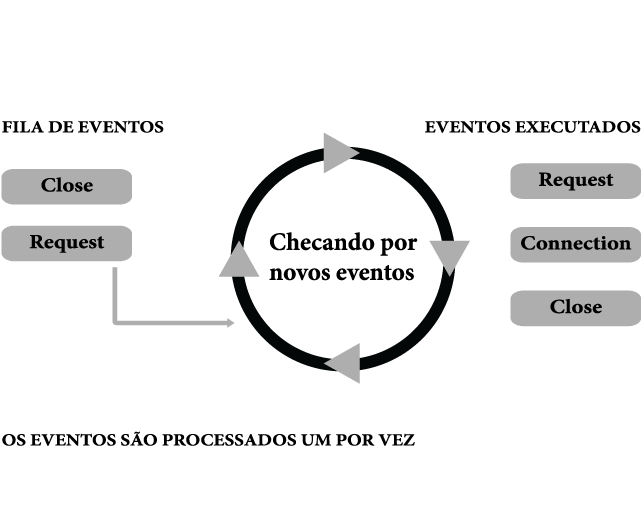
\includegraphics[width=.85\textwidth]{imagem/event-loop-caio-ribeiro.png}
  % Caption centralizada
  \captionsetup{justification=centering}
  \captionfont{\small{\textbf{\\Fonte: \cite{Pereira:2013}}}}	
  \label{fig:event-loop}
  \end{figure}
  
  A figura \ref{fig:event-loop} mostra o ciclo de eventos executado em uma repetição, recebendo o evento \textit{request}.
  
  \cite{Wilson:2013} escreve uma das qualidades do JavaScript, que foi criado seguindo o modelo de programação orientado 
  a eventos. Sendo desde um simples clique de mouse, carregamento de páginas ou envio de formulários, todos utilizando 
  o modelo baseado em eventos.
  
  O \textit{event loop} (cilo de eventos) é o sistema que usa o JavaScript para lidar com os pedidos recebidos de várias
  partes do sistema de uma forma sadia. Há uma série de maneiras como as pessoas lidam com o tempo real ou questões 
  paralelas em computação. 

  
  O JavaScript tem uma abordagem simples que torna o processo muito mais compreensível, mas introduz algumas restrições. 
  Possuindo uma ideia de como o ciclo de eventos funciona, o desenvolvedor é capaz de usá-lo em toda sua potencialidade, 
  conseguindo vantagens e evitando armadilhas dessa abordagem.\cite{Hughes:2012}
  
  Pensamos que a maioria das pessoas entendem intuitivamente a programação orientada a eventos, porquê é como a 
  vida cotidiana onde cada solicitação de evento necessita de um retorno. A programação orientada a eventos faz a 
  mesma coisa. Ao permitir que o desenvolvedor escreva código que só trabalhe em um retorno de chamada de cada vez, 
  o programa será compreensível e também capaz de executar rapidamente várias tarefas de forma eficiente.\cite{Hughes:2012}
  
  Como apresentado por \cite{Pereira:2013} o EventEmitter, é o módulo responsável por por emitir estes eventos e em 
  grande maioria das bibliotecas do ambiente Node.Js utiliza as funcionalidades de eventos deste módulo. 
  No processo de execução do evento pode-se programar qualquer lógica de programação através do 
  mecanismo de chamada de retorno. Tal chamada de retorno pode ser executado através de uma função de escuta, 
  semanticamente conhecida pelo on().
  
  Essa seção é bem descrita e exemplificada por \cite{Wilson:2013} em seu livro que nos mostra o uso e o 
  desenvolvimento de eventos.

  
  Finalizando o ciclo de eventos seção, \cite{Pereira:2013} diz que a programação orientada a eventos do Node.Js 
  foi inspirado pelos \textit{frameworks} Event Machine\footnote{http://rubyeventmachine.com/} do 
  Ruby\footnote{https://www.ruby-lang.org/en/} e Twisted\footnote{https://twistedmatrix.com/trac/} do 
  Python\footnote{https://www.python.org/}, porém o ciclo de eventos do Node.Js é mais perfomático pois seu mecanismo 
  é nativamente executado de forma não bloqueante sendo o diferencial em relação a outros ambientes de programação.
  
\section{Por que usar assíncrono}
\label{porque-usar-assincrono}

  No ambiente de desenvolvimento Node.Js é importante entender e saber trabalhar com as chamadas assíncronas. 
  \cite{Pereira:2013} em seu livro exemplifica em código as diferenças entre uma função síncrona e assíncrona 
  em relação ao tempo em que são executadas. Este código nada mais é que uma repetição de 5 interações e a cada 
  iteração desta repetição será criado um arquivo texto.
  
  Veja o tempo gasto utilizando o modelo síncrono da função \textit{fs.writeFileSync}.
  
  \begin{figure}[H]
  % Alterar espaçamentos antes e depois do caption
  \setlength{\abovecaptionskip}{0pt}
  \setlength{\belowcaptionskip}{0pt}
  % Caption
  \caption[Tempo de resposta, metódo síncrono bloqueante]{Tempo de resposta, metódo síncrono bloqueante}
  \centering
  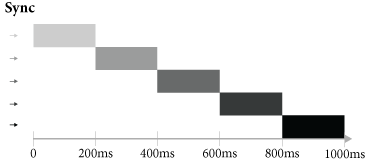
\includegraphics[width=.85\textwidth]{imagem/timeline-node-sync-caio-ribeiro.png}
  % Caption centralizada
  \captionsetup{justification=centering}
  \captionfont{\small{\textbf{\\Fonte: \cite{Pereira:2013}}}}	
  \label{fig:timeline-sync}
  \end{figure}
  
  A Figura \ref{fig:timeline-sync} exibe um quadro com um tempo de 200 ms de resposta para cada um dos 5 arquivos.

  \begin{figure}[H]
  % Alterar espaçamentos antes e depois do caption
  \setlength{\abovecaptionskip}{0pt}
  \setlength{\belowcaptionskip}{0pt}
  % Caption
  \caption[Tempo de resposta, metódo assíncrono não-bloqueante]{Tempo de resposta, metódo assíncrono não-bloqueante}
  \centering
  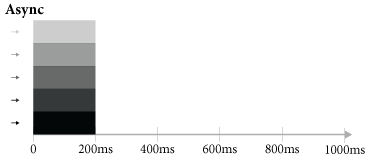
\includegraphics[width=.85\textwidth]{imagem/timeline-node-async-caio-ribeiro.png}
  % Caption centralizada
  \captionsetup{justification=centering}
  \captionfont{\small{\textbf{\\Fonte: \cite{Pereira:2013}}}}	
  \label{fig:timeline-async}
  \end{figure}

  
  Agora na Figura \ref{fig:timeline-async} o tempo total de duração foram de 200 milesegundos, pois foram executados
  de forma assíncrona maximizando o processamento.

\section{Framework Express}
\label{framework-express}

  \cite{Powers:2012} descreve que no geral um \textit{framework} ajuda na infraestrutura e que nos permite criar sites e aplicações
  com agilidade, fornecendo ao desenvolvedor um esqueleto capaz de oferecer um suporte no processo de desenvolvimento de
  software. Com os \textit{frameworks} foca-se na criação de funcionalidades da nossa aplicação ou site e 
  também fornece coesão ao código, o que nos beneficia com legibilidade e manutenabilidade.

  \cite{Pereira:2013} complementa que utilizar a API HTTP nativa do Node.Js pode ser um processo moroso e desgastante
  para o desenvolvedor. 
  Conforme surgem novas necessidades de implementação e novas funcionalidades serão acrescidas,
  os códigos se tornarão gigantescos aumentando a complexidade do projeto e dificultando futuras manutenções.
  
  Assim surge o \textit{framework} Express.Js para solucionar necessidades e agilizar no desenvolvimento.
  
  \citeonline{Powers:2012} compara que o \textit{Express.Js} é parecido com o \textit{framework} Sinatra porém bem mais \textit{RESTFUL}. 
  Pereira(2012) reafirma e complementa que o módulo \textit{Express.Js} foi inspirado pelo \textit{framework} Sinatra da 
  linguagem Ruby e que é bastante utilizado em aplicações web de grande escala.
  
  Suas características são descritas por \citeonline{Pereira:2013}:
  
  \begin{compactitem}
    \item[a)] \ac{MVR};   
    
    \item[b)] \ac{MVC};
    
    \item[c)] Roteamento de \ac{URL} com chamadas de retorno;
    
    \item[d)] Middleware;
    
    \item[e)] Interface \ac{REST};
    
    \item[f)] Suporte a File Uploads.
    
    \item[g)] Configuração baseada em variáveis de ambiente;
    
    \item[h)] Suporte a helpers dinâmicos;
    
    \item[i)] Integração com Templates Enginies;
    
    \item[j)] Integração com SQL e NoSQL;
    
  \end{compactitem}
  
  Ao criar um esqueleto utilizando o \textit{Express.js} é importante ter conhecimento do que cada
  arquivo ou diretório representa. \cite{Powers:2012, Hughes:2012} não apresentam um descritivo de cada arquivo 
  ou diretório e seu papel. Entretanto \cite{Pereira:2013, Wilson:2013} aprofundam mais neste assunto que podem ser vistos
  no \ref{apend:express-skel}.
  
  O arquivo de \textit{package.json}, de acordo com \citeonline{Wilson:2013} sempre é necessário ser criado 
  em seu projeto e que ele é responsável por fornecer detalhes sobre as condições de operação e configuração 
  esperadas por seu código. \cite{Wilson:2013} complementa que este arquivo ajuda a prevenir que alterações 
  futuras em módulos de terceiros quebrem a lógica da aplicação.

  No livro, \cite{Wilson:2013} exibe um exemplo do arquivo 
  \textit{package.json} o qual é utilizado para sincronizar a aplicação com dependências, sendo importante associar 
  a aplicação a uma versão especifica. 
  
  Para maiores detalhes sobre as notações semânticas utilizada pelo \ac{NPM} visite a documentação \cite{Semver:2013}.

\subsection{O servidor web com \textit{Express.Js}}
\label{servidor-web-express-js}

  
  De acordo com \cite{Wilson:2013} o interessante do Node.Js é que o código do 
  programa que se escreve para ele também é a implementação do servidor. 
  Seguindo este modelo tem-se a expectativa de que a aplicação funcione e se comporte de modo semelhante 
  ao ambiente de produção assim como no desenvolvimento, pois não existe nenhuma biblioteca, nenhum intermediário 
  ou \textit{daemon} que esteja no caminho.
  
  O arquivo app.js criado pelo \textit{Express.js} é em suma pequeno mas com grandes funcionalidades inclusas como 
  roteamento para solicitações \ac{HTTP} entrantes, motores de visões para renderizar marcações do HTML5
  e também download dos arquivos estáticos.

% Nome do capítulo
\chapter{Metodologia}
% Label para referenciar
\label{metodologia}

% Diminuir espaçamento entre título e texto
\vspace{-1.9cm}

% Texto do capítulo
  Baseando-se em metodologias de desenvolvimento de software ágil Scrum, foram determinadas 
  as seguintes etapas para elaboração deste trabalho:


\section{Estudo do ambiente Node.Js}
  
  \begin{compactitem}
    \item[a)] Estudar o paradigma de orientação a eventos.
    \item[b)] Estudar o Event Loop.
    
    Busca um entendimento básico sobre o ciclo de eventos (Event-Loop) e como ele é utilizado no NodeJs.
    
    \item[c)] Estudar as principais características do Node.Js.
    
    Conhecer o modelo single-thread, diferenças entre o modelo assíncrono e síncrono, dentre outros.
    
    \item[d)] Estudo do framework Express
    
    Conhecer o framework feito em Node.Js que será a base para criar a 
    aplicação devido a grandes módulos já inclusos e se codificar de maneira \ac{REST}.

  \end{compactitem}
  
\section{Levantamento de requisitos}

  \begin{compactitem}
    \item[a)] Estudar a arquitetura web
    
    Buscando um entendimento básico de como é a implementação de uma aplicação 
    \ac{REST} e seus protocolos relacionados ao HTTP.
    
    \item[b)] Especificar requisitos da aplicação.
    
    Criar um modelo de \ac{API} da aplicação para fácil entendimento e
    independente da plataforma de desenvolvimento.
    
    \item[c)] Especificar serviços da aplicação.
    
    Detalhar e documentar o serviço de hospedagem na internet, além de outros componentes 
    necessários para o funcionamento do ecossistema da aplicação como:
    
      \begin{compactitem}
	\item[-] Hardware utilizado;
	\item[-] Servidor web para responder requisições na porta 80;
	\item[-] Serviços adicionais instalados ( Banco de dados );
	\item[-] Softwares para monitorar desempenho e utilização do servidor;
      \end{compactitem}
      
  \end{compactitem}

\section{Criar dois aplicativos em diferentes paradigmas}
  
  \begin{compactitem}
    \item[a)] Desenvolvimento da aplicação no paradigma orientado a eventos.
    
    Desenvolver um aplicativo escrito no ambiente Node.Js com o framework Express.Js
    
    \item[b)] Desenvolvimento do mesmo aplicativo em outros ambientes.
    
    Busca-se com esta etapa ter um aplicativo escrito na linguagem Python com o framework Django
    para comparamos o desempenho, do ambiente aqui estudado.
    
  \end{compactitem}

\section{Especificar testes e comparar resultados}

  \begin{compactitem}
    \item[a)] Utilizar testes de carga na \ac{API}.
    
    Realizar um plano de testes de estresse e carga nas \ac{API} desenvolvidas através
    da ferramenta loader.io \footnote{\label{noteloader}http://loader.io}, melhor descrita na Sub-Seção \ref{ferramentas-utilizadas-para-testes}.
    
    
    \item[b)] Descrever o software de testes.
    
    Descrever passo a passo como gerar um teste de carga na aplicação dos serviços descritos acima.
    
    \item[c)] Executar os testes para avaliar o desempenho das aplicações.
    
    Executar os testes para obter informações e medir o desempenho de cada aplicação.
    
    \item[d)] Avaliar os resultados obtidos após a analise, coleta e definições das métricas.
    
    Por último realizar uma análise sobre o desempenho positivo ou negativo de cada modelo desenvolvido.
    
%    Definir aqui as métricas passadas pelo serviço web loader.io.
    
  \end{compactitem}

% testes de carga: Testes realizados para verificar se um sistema suporta uma determinadas
% carga. Volume do trafego para um determinado sistema. Geralmetne medida em transacoes
% requisicoes dos ususarios

% Transação: operação completa no sistema. Por exemplo, buscar um produto.
% Sistema: todo o conjunto de servidores, rede entre servidores, softwares de terceiros e a aplicação.
% Utilização de um recurso: percentual, em uso, do total de recursos disponíveis.
% Tempo de resposta: Tempo desde o momento em que o usuário envia a requisição até o momento em que recebe a resposta completa.
% Na nomeclatura do Jmeter , é o elapsed time

% Profiling: instrumentação da aplicação para estudo dos métodos e seus tempos de execução.
% Vazão: taxa com que um sistema responde às requisições recebidas.
% Gargalo: tudo o que impede que o sistema apresente maior vazão.
% Se a vazão for inferior à taxa com que as requisições são enviadas ao sistema.

% Monitoramento do sistema
% Métricas Sistema Operacional (Todas as máquinas)
% Utilização CPU, memória, Swap, disco, rede, etc.
% /proc, perfmon, vmstat, etc.

% Métricas Banco de Dados
% Tempo ocupado, tempo execução médio por query, locks, leituras físicas e lógicas, etc.
% Relatório AWR, etc.

% Profiling(Servidor de aplicação)
% Tempo de execução por método, tempo de execução em CPU por método, memória consumida por classe, etc.
% VisualVM, RedGate Ants, etc.

% NewRelic
% Integra profiling e monitoramento de métricas do sistema operacional.

% testes de estresse: Testes realizados para determinar
% a capacidade maxima do sistema.

\subsection{Ferramentas Utilizadas}
\label{ferramentas-utilizadas-para-testes}
  
  Para realizar os testes de carga e estresse será utilizado o serviço em computação nas nuvens
  da empresa SendGrid\footnote{http://labs.sendgrid.com/} denominado loader.io.
  
  De acordo com o sitio o serviço é definido com um serviço de teste de carga livre,
  que permite realizar testes de estresse em aplicativos web ou \ac{API} com milhares de conexões simultâneas
  (tradução nossa).
  
  Na documentação\footnote{http://support.loader.io/} do serviço, mais especificamente, na seção começando (tradução nossa)
  temos as seções de como criar o teste, tipos de teste, verificando um aplicativo, variáveis,
  resultados de testes(tradução nossa). Neste capítulo não iremos abordar todos os items pois serão melhor explicados
  no Capítulo \ref{}. Apenas a seção tipos de testes será explicada neste momento.
  
  Os três tipos de testes suportados pelo serviço são:
  
  Clientes por testes
  
  Este teste permite que especifique um número total de clientes que se conectam ao serviço. Quando criar o teste,
  especifique somente um número de clientes então vários clientes irão se conectar ao longo da duração do teste. 
  Por exemplo, se for criado um teste com 20.000 clientes dentro de 20 segundos, o serviço irá executar a carga de 
  1.000 clientes por segundo. (tradução nossa)
  
  Clientes por segundo
  
  Este teste permite que especifique um número de clientes que se conectam a cada segundo. Por exemplo se for criado
  um teste com 1.000 clientes dentro de 20 segundos, o serviço irá conectar 20.000 clientes por teste.
  
  Mantendo carga do clientes
  
  Segundo a definição da documentação, este teste é utilizado para sobrecarregar (martelar) o site ou \ac{API}.
  
  O serviço loader.io garante que um número constante de clientes estará consumindo e realizando requisições em 
  sua \ac{API} a todo o momento.
  
  Este teste permite que especifique um número mínimo e máximo de clientes. Especificando zero clientes
  até 10.000, por exemplo, o teste vai começar com zero até 10.000 clientes simultâneos no final do teste.
  



\chapter{Desenvolvimento dos protótipos}
% Label para referenciar
\label{desenvolvimento-prototipos}

% Diminuir espaçamento entre título e texto
\vspace{-1.9cm}

% Texto do capítulo

  Este capítulo apresenta o cenário proposto para o estudo de caso, bem
  como o desenvolvimento dos protótipos com suas fases de implementação, iniciando
  pela elicitação dos requisitos seguindo a abordagem \ac{REST}.
  
  Como serão desenvolvidos dois protótipos com o objetivo de compara-los um com o outro,
  iniciaremos o desenvolvimento com o \textit{framework} Django e por fim faremos o desenvolvimento
  com o ambiente Node.Js e \textit{framework} Express.Js formando assim a aplicação proposta
  
\section{O escopo do projeto}
\label{escopo-projeto}

  Com base nos aspectos abordados ao longo deste trabalho, 
  esta seção visa apresentar o desenvolvimento de um Web Service seguindo os padrões \ac{REST} e a utilização 
  de um banco de dados relacional Postgres para a persistência dos dados.
  
  Tal serviço possuirá métodos que serão consumidos por dispositivos clientes.

\subsection{Levantamento Requisitos}
\label{levantamento-requisitos}

  Utilizaremos o mesmo exemplo citado por \citeonline{Pereira:2013} pois é de fácil compreensão
  e entendimento de uma simples aplicação.

\subsubsection{Elicitação de requisitos}

  É possível destacar os seguintes requisitos candidatos

  \begin{compactitem}
    \item[a)] Não utilizar técnicas de autenticação na API.
    \item[b)] A \ac{API} \ac{REST} deverá responder as requisições do cliente através da representação em JSON.
    \item[c)] A \ac{API} \ac{REST} deverá persistir os dados em Postgres.
    \item[d)] A \ac{API} \ac{REST} deverá ter um recurso chamado Pessoas.
    \item[e)] A \ac{API} \ac{REST} deverá prover estratégias para manipular as ações de CRUD de uma pessoa(s)
    \item[f)] A \ac{API} \ac{REST} deverá ter um recurso chamado Contatos.
    \item[g)] A \ac{API} \ac{REST} deverá prover estratégias para manipular as ações de CRUD de um contato(s)
  \end{compactitem}
  
\subsubsection{Análise dos requisitos}
  
  Perante os requisitos elicitados verificou-se que o objetivo essencial de uma pessoa, candidato a usuário
  do sistema, é controlar os própios contatos.
  
  O principal requisito destacado na análise é registrar estes contatos. Para atender o requisito
  propoem-se a utilização de uma \ac{API} \ac{REST}, para fornecer os \ac{CRUD} de cada recurso
  como na Tabela \ref{tab:api-descricao-contato}.
 
  
  \begin{table}[H]
    \centering
    \footnotesize
    \vspace{0.5cm}
    % Alterar espaçamentos antes e depois do caption
    \setlength{\abovecaptionskip}{0pt}
    \setlength{\belowcaptionskip}{0pt}
    % Caption
    \caption[Descrição da API de contatos]{Descrição da API de contatos}
    \label{tab:api-descricao-contato}
    % Conteúdo da tabela
    \begin{tabular}{c|c|c|p{8cm}}
      \hline \hline
      Metódo  &	Parâmetro &	Recurso &	Descrição \\
      \hline \hline
      GET	& -	& contatos	& Retorna a lista de contatos 
					  cadastrados no banco de dados \\
      \hline \hline
    \end{tabular}
    % Fonte
    \captionfont{\small{\textbf{\\Fonte: Autor}}}
  \end{table}
  
\subsubsection{Tecnologias Utilizadas}


  Aplicativo comparativo Django
    
    \begin{compactitem}
      \item[a)] Python – Linguagem de programação OO usada na comparação de aplicativos deste trabalho;
      \item[b)] Postgress – Banco de dados relacional
      \item[c)] Django/django-rest-framework – Framework Django para aplicações web e o pacote django-rest-framework
      para facilitar o desenvolvimento.
    \end{compactitem}
    
  Aplicativo Node.JS
  
    \begin{compactitem}
      \item[a)] Node.Js – Ambiente de Programação Backend para apresentação deste trabalho
      \item[b)] Postgress – Banco de dados relacional
      \item[c)] Express – Framework para aplicações web
    \end{compactitem}
  
  Para os protótipos temos as principais tabelas, chamada de person e contact,
  que faz o registro de pessoas e contatos, respectivamente, e possui os atributos (campos) necessários
  para armazenar os registros da API no banco de dados. Na entidade de person, temos um identificador
  "id" único e auto-incremento, "created" e "modified" como campos de data e o campo
  "nome" para identicar quem é a pessoa. Na tabela de contact temos um identificador "id" único e auto-incremento,
  "created" e "modified" como campos de data, "kind" com caracter para saber o tipo do contato e "value" para 
  saber o valor do tipo do contato. A tabela "contact" possui uma relação com a tabela "person", coforme a Figura 
  \ref{fig:der}, com cardinalidade de muitos para um.

  \begin{figure}[H]
  % Alterar espaçamentos antes e depois do caption
  \setlength{\abovecaptionskip}{0pt}
  \setlength{\belowcaptionskip}{0pt}
  % Caption
  \caption[Diagrama de entidade e relacionamentos]{Diagrama de entidade e relacionamentos}
  \centering
  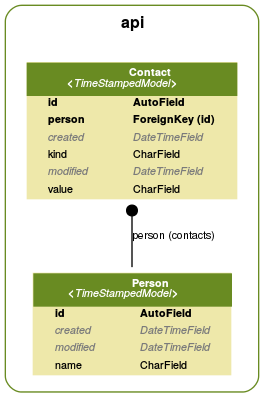
\includegraphics[width=.55\textwidth]{imagem/der.png}
  % Caption centralizada
  \captionsetup{justification=centering}
  \captionfont{\small{\textbf{\\Fonte: Autor}}}	
  \label{fig:der}
  \end{figure}
  
\section{Aplicação em Django}
\label{desenvolvimento-django}

  Falta algum texto

\section{Aplicação em Express.Js}
\label{escopo-projeto}

  Falta algum texto


\chapter{Experimentos e resultados}
% Label para referenciar
\label{experimentos-resultados}

% Diminuir espaçamento entre título e texto
\vspace{-1.9cm}

% Texto do capítulo

 Neste capítulo vamos abordar o ambiente de testes para os nossos protótipos e apresentar 
 o plano de testes utilizado e os resultados obtidos e análise dos dados.

\section{Ambiente de testes}
\label{ambientedetestes}

  Para efetuar os testes, os protótipos tiveram de ser colocados em uma ambiente de testes. 
  Para os dois protótipos, hospedamos a aplicação em uma VPS\footnote{http://digitalocean.com} da empresa Digital Ocean.
  
  O ambiente é composto pelos seguintes componentes de hardware conforme descrito nas tabelas\footnote{https://www.digitalocean.com/pricing/}
  de precificação do produto.
  
  \begin{table}[H]
    \centering
    \footnotesize
    % Alterar espaçamentos antes e depois do caption
    \setlength{\abovecaptionskip}{0pt}
    \setlength{\belowcaptionskip}{0pt}
    % Caption
    \caption[Componentes da VPS]{Componentes da VPS}
    \label{tab:components-digital-ocean-vps}
    % Conteúdo da tabela
    \begin{tabular}{c|c}
      \hline \hline
      Componente  &	Descrição \\
      \hline \hline
      Memória Ram & 512 MegaBytes \\
      Processador & 1 núcleo. \\
      Espaço em disco & 20 GigaBytes \ac{SSD}. \\
      Transferência em rede & 1 TeraByte. \\
      \hline \hline
    \end{tabular}
    % Fonte
    \captionfont{\small{\textbf{\\Fonte: Digital Ocean Pricing <https://www.digitalocean.com/pricing/> acesso 05. NOV. 2014}}}
  \end{table}

  Para os dois protótipos busca-se manter o máximo de igualdade entre os serviços executados, porém, por ser 
  tecnologias diferentes o modo de \textit{deploy} também são diferentes adicionando ou não novos serviços. 
  As informações dos serviços executados está listada de acordo com o software de monitoramento\footnote{http://newrelic.com}
  da empresa New Relic.
  
  A tabela \ref{tab:services-in-api-django} apresenta os serviços em execução do protótipo feito em Django sem clientes conectados.
  Este ambiente é composto por um servidor Nginx a execução do \textit{gunicorn},
  que nada mais é a execução do framework Django, o banco de dados Postgres 9.1 e o processo supervisord responsável por
  verificar se a aplicação esta ativa e caso ocorra alguma falha é capaz de reiniciar a aplicação.
  
  \begin{table}[H]
    \centering
    \footnotesize
    % Alterar espaçamentos antes e depois do caption
    \setlength{\abovecaptionskip}{0pt}
    \setlength{\belowcaptionskip}{0pt}
    % Caption
    \caption[Serviços executados na API Django]{Serviços executados na API Django}
    \label{tab:services-in-api-django}
    % Conteúdo da tabela
    \begin{tabular}{c|c|c}
      \hline \hline
      Processo  & 	CPU \% &	Memória \\
      \hline \hline
      gunicorn &	0.0\% &		104 MB \\
      postgres &	0.0\% &		19.3 MB \\
      supervisord &	0.0\% &		11.5 MB \\
      nginx &		0.0\% &		7.26 MB \\
      getty &		0.0\% &		5.69 MB \\
      udevd &		0.0\% &		4.05 MB \\
      nrsysmond &	0.1\% &		3.93 MB \\
      console-kit-dae &	0.0\% &		3.84 MB \\
      polkitd &	 	0.0\% &		2.98 MB \\
      ntpd &		0.0\% &		2.34 MB \\
      rsyslogd &	0.0\% &		1.47 MB \\
      nginx &		0.0\% &		1.38 MB \\
      sshd &		0.0\% &		1.22 MB \\
      dbus-daemon &	0.0\% &		1.13 MB \\
      cron &		0.0\% &		1.03 MB \\
      exim4 &		0.0\% &		992 KB \\
      init &		0.0\% &		820 KB \\
      acpid &		0.0\% &		656 KB \\
      atd &		0.0\% &		156 KB \\
      su &		0.0\% &		0 \\
      bash &		0.0\% &		0 \\
      \hline \hline
    \end{tabular}
    % Fonte
    \captionfont{\small{\textbf{\\Fonte: Autor}}}
  \end{table}
  
  \vspace{-1.9cm}

  Para o segundo protótipo, com Node.Js, possuimos os seguintes serviços executados na tabela \ref{tab:services-in-api-node}, 
  também sem nenhum cliente conectado. Este ambiente é composto por um servidor Nginx, o serviço \textit{pm2} responsável por
  verificar se a aplicação esta ativa e caso ocorra alguma falha é capaz de reiniciar a aplicação, 
  o banco de dados Postgres 9.1.
  
   \begin{table}[H]
    \centering
    \footnotesize
    % Alterar espaçamentos antes e depois do caption
    \setlength{\abovecaptionskip}{0pt}
    \setlength{\belowcaptionskip}{0pt}
    % Caption
    \caption[Serviços executados na API Node]{Serviços executados na API Node}
    \label{tab:services-in-api-node}
    % Conteúdo da tabela
    \begin{tabular}{c|c|c}
      \hline \hline
      Processo  & 	CPU \% &	Memória \\
      \hline \hline
      node &		0.0\% &		22.8 MB \\
      postgres &	0.0\% &		17.8 MB \\
      pm2 &		0.0\% &		17.4 MB \\
      nginx &		0.0\% &		6.61 MB \\
      getty &		0.0\% &		5.68 MB \\
      udevd &		0.0\% &		3.72 MB \\
      nrsysmond &	0.1\% &		3.93 MB \\
      rsyslogd &	0.0\% &		1.52 MB \\
      nginx &		0.0\% &		1.38 MB \\
      sshd &		0.0\% &		1.22 MB \\
      cron &		0.0\% &		1.02 MB \\
      exim4 &		0.0\% &		984 KB \\
      init &		0.0\% &		824 KB \\
      acpid &		0.0\% &		652 KB \\
      dbus-daemon &	0.0\% &		508 KB \\
      atd &		0.0\% &		152 KB \\
      su &		0.0\% &		0 MB \\
      console-kit-dae &	0.0\% &		0 MB \\
      startpar & 	0.0\% &		0 MB \\
      sshd &		0.0\% &		0 MB \\
      polkitd &		0.0\% &		0 MB \\
      \hline \hline
    \end{tabular}
    % Fonte
    \captionfont{\small{\textbf{\\Fonte: Autor}}}
  \end{table}
   
\subsection{Apresentação da ferramenta}
  
  Para realizar a simulação de múltiplos usuários na \ac{API} e obter os dados dos testes foi 
  escolhido o software como serviço da empresa SendGrid chamado loader.io. O loader.io é descrito em seu site
  como um simples serviço de teste de carga baseado em núvem (tradução nossa). Em sua descição tem-se a seguinte
  definição: Loader.io é um serviço de teste de carga, livre, que permite realizar um teste de estresse em 
  seus aplicativos web ou \textit{api\'s} com milhares de conexões simultâneas (tradução nossa).
  
  Sua utilização é simples, basta criar uma conta com um e-mail válido. Após o e-mail ser validado pode-se 
  criar um teste dentre os 03 tipos já apresentados. Em resumo, temos os seguintes campos a serem preenchidos:
  
  \textbf{Nome do teste}: Nome dado ao teste para ser encontrado com maior facilidade;
  Tipo de teste: São apenas 03 tipos suportados pelo serviço. Clientes por teste, Clientes por segundo e Mantendo 
  a carga no servidor.
  
  \textbf{Autenticação}: Caso sua aplicação necessite de autenticação escolha a opção Autenticação Básica (tradução nossa),
  e setar os valores dos campos usuário e senha (tradução nossa). O serviço loader.io pede atenção 
  pois os campos, usuário e senha, não serão criptografados. Então é recomendado criar um usuário de teste na aplicação.
  
  \textbf{Conexões e Duração}: São as principais definições para o teste sendo que o campo duração
  é fixo em 60 segundos. As conexões serão explicadas na próxima sub-seção em conjunto com os tipos de teste.
  
  \textbf{Tempo limite e Erro}: Este campo especifica quanto tempo o teste irá esperar por uma resposta do aplicativo, antes
  de contar a requisição como erro. Por padrão é configurado para 10000 milessegundos ou 10 segundos.
  
  \textbf{Notas e etiquetas}: São campos para o desenvolvedor descrever  melhor os testes.
  
  \textbf{Urls e opções}: Configura a \ac{URL} que se deseja testar. Ha outras opções disponíveis como setar cabeçalhos \ac{HTTP},
  opções de resposta, váriaveis e outros que não serão utilizados neste trabalho.
  
  Para melhor entendimento do leitor e detalhamento é importante verificar 
  a documentação \footnote{http://support.loader.io/article/15-creating-a-test}.
  
\subsubsection{Tipos de teste}
  
  Os três tipos de testes suportados pelo serviço são:
  
  \textbf{Clientes por testes}
  
  Este teste permite que especifique um número total de clientes que se conectam ao serviço. Quando criar o teste,
  especifique somente um número de clientes então vários clientes irão se conectar ao longo da duração do teste. 
  Por exemplo, se for criado um teste com 20.000 clientes dentro de 20 segundos, o serviço irá executar a carga de 
  1.000 clientes por segundo. (tradução nossa)
  
  Em referência ao formulário de criação de teste o campo clientes representa o número de conexões que serão
  feitas para o servidor ao longo da duração do teste.
  
  \textbf{Clientes por segundo}
  
  Este teste permite que especifique um número de clientes que se conectam a cada segundo. Por exemplo se for criado
  um teste com 1.000 clientes dentro de 20 segundos, o serviço irá conectar 20.000 clientes por teste.
  
  Em referência ao formulário de criação de teste o campo clientes representa o número de conexões que serão
  feitas para o servidor por segundo.
  
  \textbf{Mantendo carga do clientes}
  
  Segundo a definição da documentação, este teste é utilizado para sobrecarregar o site ou \ac{API}.
  
  O serviço loader.io garante que um número constante de clientes estará consumindo e realizando requisições em 
  sua \ac{API} a todo o momento.
  
  O teste inicia-se com um certo número de conexões ("de")  e pode aumentar as conexões ao longo do teste, 
  atingindo o número no campo "para", até ao final do teste. 
  
  Este teste permite que especifique um número mínimo e máximo de clientes. Especificando zero clientes
  até 10.000, por exemplo, o teste vai começar com zero até 10.000 clientes simultâneos no final do teste.
  
\subsubsection{Verificando o aplicativo}

  Após ter um entendimento base sobre os testes e como cadastra-los é necessário verficar a autenticidade do 
  aplicativo ou domínio para com o serviço Loader.io. Este processo só é feito uma vez. 
  
  O token fornecido pelo Loader.io pode ser verificado de duas maneiras.
  
  \textbf{Verificação por HTTP}.
  
  Pode-se realizar upload do arquivo loader-\textit{token} para o aplicativo e fazer com que a aplicação
  responda este arquivo texto através de uma rota com o mesmo nome do arquivo. 
  
  Para este trabalho, não foi feito upload do arquivo. Em vez disso, criamos a rota com o nome do token e
  na resposta da requisição \ac{HTTP} alteramos o cabeçalho do protocolo para \textit{text/plain} e imprimimos
  o valor do token.
  
  \textbf{Verificação por DNS.}
  
  A verificação ocorre quando o valor do token é inserido nas configurações de hospedagem através de um
  registro txt, com o valor \textit{loaderio=token}.
  
  Lembrando ao leitor que a propagação do \ac{DNS} pode levar algum tempo.
  
\subsubsection{Variáveis no Loader.io}

  As variáveis permitem usar dados de um cabeçalho de resposta \ac{HTTP} anterior e passa-los para o próximo
  teste.
  
  Como no exemplo da documentação do loader.io, em uma requisição do tipo \textit{GET} foi configurada uma váriavel
  com a chave \ac{CSRF} e o respectivo valor de cabeçalho \textit{X-Csrf-Token}. Em seguida em uma requisição 
  do tipo \textit{POST} foi utilizada essa chave-valor através da variável com o nome \textit{authenticity token} e valor
  \textit{\{\{csrf\}\}}.
  
  Essa opção de uso de váriaveis não foi utilizada em nossos testes mas é importante relatar ao leitor que
  é existe tais funcionalidades na ferramenta.

  
\subsubsection{Resultados dos testes}

  Para cada execução de teste gera-se um resultado. Veja abaixo um sumário de cada campo para melhor interpretação.
  
  \begin{compactitem}
    \item[a)] Date e Time: Data e hora de quando o teste foi executado.
    \item[b)] Max users: Número máximo de conexões que foram feitas.
    \item[a)] Duration:  Duração do teste.
    \item[a)] Success response: O número total de resposta com staus code (1xx,2xx,3xx).
    \item[a)] Avg responses time: Tempo médio que o aplicativo esperou por uma resposta do aplicativo.
    \item[a)] Sent from app: Quantidade total em MegaBytes enviados para o aplicativo.
    \item[a)] RCVD from loader: Quantidade total em MegaBytes foi recebida pelo aplicativo.
    \item[a)] Timeout errors: Número de pedidos que não receberam uma resposta dentro do tempo limite configurado.
    \item[a)] Network errors: Erros da camada de transporte e de rede como \ac{DNS}, \textit{timeouts} de conexão TCP, dentre outros.
    \item[a)] Errors(400/500): Respostas das requisições com um código de erro (4xx e 5xx).
    \item[a)] Avg error rate: Porcentagem de erros do total de tentativas dos pedidos.
  \end{compactitem}

  \textbf{Gráficos}
  
  São três tipos de gráficos disponibilizados pelo Loader.io que oferecem informações mais detalhadas 
  sobre o que ocorreu na execução do teste como tempos de resposta, taxas de erro e largura de banda.
  
  \textbf{O gráfico temporal}.
  
  Gráfico que exibe os tempos de resposta apresentando duas linhas.
  
  Em verde, tem-se o número de conexões realizadas no aplicativo. E em azul é o tempo médio de resposta das
  requisições.
  
  \textbf{O gráfico de detalhes.}
  
  O gráfico que exibe taxas de sucesso e também de erros. Seu objetivo é exibir quando o aplicativo
  começa a disparar os erros.
  
  \textbf{O gráfico largura de banda.}
  
  Este gráfico mostra o quanto os dados foram enviados a partir do seu aplicativo.


\section{Testes}

  Descreve-se nesta seção os planos de testes utilizado em cada tipo de teste e a interpretação dos seus resultados
  através de comparação.
  
  Foi utilizada a seguinte nomenclatura para os testes com o aplicativo Django. Primeiramente teremos a letra (A) para identificar
  que o plano de teste será executado para o aplicativo Django. Em seguida temos a sequência númerica de 01 a 03, 
  identificando o testes realizados. 
  
  No aplicativo Node.Js utilizamos o mesmo padrão descrito no paragráfo anterior alterando apenas a letra inicial para (B) identificando
  que os testes foram realizados para o aplicativo em Node.Js
  Para melhor visualização dos resultados vamos sumarizar todos os testes em uma nova tabela e gerar um gráfico para apresentar
  os dados ao leitor.
    
\subsection{Manter a carga no Servidor}  

    
  Apresenta-se nesta seção o plano de teste A-3 e B-3 que corresponde ao teste manter carga de usuários o qual tem-se um sumário
  com as médias de cada execução.
  
  Para melhor instruir o leitor, esse teste inicia com 50 a 100 usuários conectados no sistema até 1 minuto de duração. Para cada teste
  foi executado 7 vezes e destes resultados retiramos a média para o tempo de resposta, número de sucessos, erro de tempo de limite e
  e a média para erros de rede. No decorrer da série acrescentamos 50 usuários até a quantidade máxima suportada pela aplicação.
  
  Veja o exemplo do teste A-3.1 o qual obtivemos os dados gerados pela ferramenta.
  
  \begin{table}[H]
    \centering
    \footnotesize
    % Alterar espaçamentos antes e depois do caption
    \setlength{\abovecaptionskip}{0pt}
    \setlength{\belowcaptionskip}{0pt}
    % Caption
    \caption[Teste A-3.1 com a API Django 50 – 100 clientes]{Teste A 3.1 com a API Django 50 – 100 clientes}
    \label{tab:teste-a-3-1}
    % Conteúdo da tabela
    \begin{tabular}{c|c|c|c|c}
      \hline \hline
      Número de execução &	Tempo médio de resposta &	Número de sucessos &	Timeout Error &		 Network Errors&	Avg Error Rate \% \\
      \hline \hline
      Primeira execução &	1605 &				2754 &			0 &				0 &		0 \\
      Segunda execução &	1661 &				2659 &			0 &				0 &		0 \\
      Terceira execução &	1691 &				2610 &			0 &				0 &		0 \\
      Quarta execução  &	1678 &				2631 &			0 &				0 &		0 \\
      Quinta execução  &	1652 &				2674 &			0 &				0 &		0 \\
      Sexta execução   &	1634 &				2712 &			0 &				0 &		0 \\
      Sétima execução  &	1628 &				2707 &			0 &				0 &		0 \\
      Media & 			1649.8571428572 &		2678.1428571429 & 	0 &				0 &		0 \\
      \hline \hline
    \end{tabular}
    % Fonte
    \captionfont{\small{\textbf{\\Fonte: Autor}}}
  \end{table}
  
  A tabela \ref{tab:teste-a-3-1} mostra que na primeira execução do teste A-3.1 com o minimo de 50 clientes até o máximo de 100 clientes
  durante 1 minuto de duração. Para este teste obteve-se 1605 milesegundos no tempo médio de resposta,
  2754 números de sucessos, 0 erros de tempo de limite, 0 erros de rede.
  
  Para este plano de teste A-3, foram realizados as séries A-3.1 de 50 a 100 clientes, A-3.2 de 100 a 150 clientes, A-3.3 de 150 a 200 clientes,
  A-3.4 de 200 a 250 clientes, A-3.5 de 250 a 300, A-3.6 de 300 e 350 clientes. Com os dados obtidos de cada teste pode-se fazer o sumário
  destes que serão apresentados a seguir na tabela \ref{tab:sumario-resultado-plano-teste-a-3}.
  
  \begin{table}[H]
    \centering
    \footnotesize
    % Alterar espaçamentos antes e depois do caption
    \setlength{\abovecaptionskip}{0pt}
    \setlength{\belowcaptionskip}{0pt}
    % Caption
    \caption[Sumário dos resultados do plano A-3]{Sumário dos resultados do plano A-3}
    \label{tab:sumario-resultado-plano-teste-a-3}
    % Conteúdo da tabela
    \begin{tabular}{c|c|c|c|c}
      \hline \hline
      Intervalos  & 	Média de tempo de resposta (ms) \% &	Número de sucessos & 	Erro de tempo de limite &	Erro de rede \\ 
      \hline \hline
      50 a 100 &		1649.8571428572 &		2678.1428571429 & 	0 &				0 \\
      100 a 150&		2663.1428571429 &		2734.2857142857 & 	2.8571428571  &			0 \\
      150 a 200&		5539.8571428572 &		1487.4285714286 & 	258.8571428571 &		0 \\
      200 a 250&		5452.2857142857 &		1714.4285714286 & 	574.4285714286 &		0 \\
      250 a 300&		5964.1428571429 &		1717.5714285714 & 	810.5714285714 &		0 \\
      300 a 350&		6256.7142857143 &		1625.8571428572 & 	935.2857142857 &		0 \\
      \hline \hline
    \end{tabular}
    % Fonte
    \captionfont{\small{\textbf{\\Fonte: Autor}}}
  \end{table}
   
  A tabela \ref{tab:sumario-resultado-plano-teste-a-3} exibe as médias dos campos (média de tempo de resposta, 
  média do número de sucessos, média de erros de tempo de limite, média de erros de rede) de cada teste executado 
  para o plano de teste A-3 do protótipo Django.
  
  Com os dados acima foi possível gerar o gráfico \ref{grafico:teste-mantendo-carga-usuario-django} do 
  prtótipo Django.
  
  \begin{grafico}[H]
    % Alterar espaçamentos antes e depois do caption
    \setlength{\abovecaptionskip}{5pt}
    \setlength{\belowcaptionskip}{0pt}
    \label{grafico:teste-mantendo-carga-usuario-django}
    % Caption
    \caption[Mantendo a carga de usuários no Django]
	    {Mantendo a carga de usuários no Django}
    \centering
    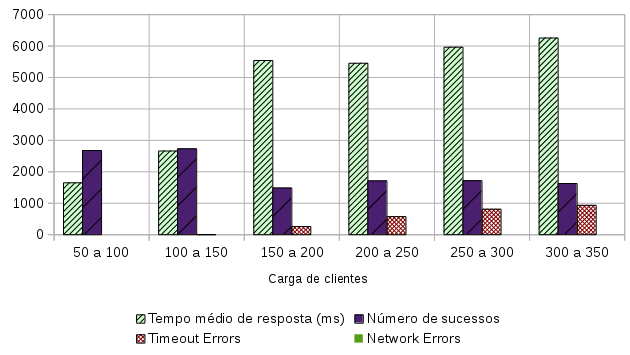
\includegraphics[width=.80\textwidth]{imagem/graficos/grafico_django_plano_de_teste_3.png}
    % Caption centralizada
    \captionsetup[grafico]{justification=centering}
    % Fonte
    \captionfont{\small{\textbf{\\Fonte: Autor}}}
  \end{grafico}
  
  Ao interpretar o gráfico \ref{grafico:teste-mantendo-carga-usuario-django}  observa-se que com baixos números de clientes 
  conectados no sistema tem-se um tempo de resposta menor para um alto número de sucessos. Ao elevar o número minimo e máximo de 
  clientes conectados observa-se que o tempo de resposta foi quase o mesmo do número de sucessos. Com novos acréscimos de usuários
  no protótipo elevando o número minimo e máximo de clientes conectados pode-se observar que o tempo médio de resposta foi elevado
  em grandes números e o número de sucessos de cada requisição abaixou em comparação ao primeiro teste. Também é possível verificar,
  que com o aumento de usuários houve a incidência de erros de tempo de limite nas conexões.
  
  Este teste prova que o protótipo Django possui pouca eficiência em lidar com usuários conectados ao sistema. Veja que os tempos de 
  resposta são altos e o número de sucessos são baixos para uma aplicação simples cujo objetivo é somente consumir as informações do banco de 
  dados através do método \textit{GET} da API.
  
  Seguindo o mesmo modelo e conceitos de teste adotado para o protótipo Django, foi aplicado no plano de teste 
  B-3 correlacionando ao protótipo Node.Js. 
  
  A partir do exemplo do teste B-3.1 o qual obtivemos os dados gerados pela ferramenta, já é possível comparar a eficiência das 
  tecnologias empregadas em cada protótipo.
  
  \begin{table}[H]
    \centering
    \footnotesize
    % Alterar espaçamentos antes e depois do caption
    \setlength{\abovecaptionskip}{0pt}
    \setlength{\belowcaptionskip}{0pt}
    % Caption
    \caption[Teste B-3.1 com a API Node.Js 50 – 100 clientes]{Teste B 3.1 com a API Node.Js 50 – 100 clientes}
    \label{tab:teste-b-3-1}
    % Conteúdo da tabela
    \begin{tabular}{c|c|c|c|c}
      \hline \hline
      Número de execução &	Tempo médio de resposta &	Número de sucessos &	Timeout Error &		 Network Errors&	Avg Error Rate \% \\
      \hline \hline
      Primeira execução &	229 &				19632 &			0 &				0 &		0 \\
      Segunda execução &	230 &				19514 &			0 &				0 &		0 \\
      Terceira execução &	233 &				19282 &			0 &				0 &		0 \\
      Quarta execução  &	230 &				19486 &			0 &				0 &		0 \\
      Quinta execução  &	235 &				19103 &			0 &				0 &		0 \\
      Sexta execução   &	231 &				19389 &			0 &				0 &		0 \\
      Sétima execução  &	240 &				18724 &			0 &				0 &		0 \\
      Media & 			232.5714285714 &		19304.2857142857 & 	0 &				0 &		0 \\
      \hline \hline
    \end{tabular}
    % Fonte
    \captionfont{\small{\textbf{\\Fonte: Autor}}}
  \end{table}
  
  A tabela \ref{tab:teste-b-3-1} mostra que na primeira execução do teste B-3.1 com o minimo de 50 clientes até o máximo de 100 clientes
  durante 1 minuto de duração. Para este teste obteve-se 232 milesegundos no tempo médio de resposta, valor muito inferior ao do plano de
  teste A-3.1 da tabela \ref{tab:teste-a-3-1} o qual foi de 1649.8571428572 milsesegundos, significando que a resposta para os usuários
  foi bem mais rápida do que o protótipo em Django. Vale ressaltar que o número de sucessos para cada conexão ficou em média de 
  19304.2857142857, número superior ao teste A-3.1 de apenas 2754 números de sucessos.
  
  Outro dado importante a ser salientado é que no plano de teste B-3 conseguiu alcançar o limite de 450 a 500 usuários conectados
  na aplicação durante 1 minuto de duração. Valor este superior ao do plano de teste A-3 em que o limite de usuário chegou a apenas
  de 300 a 350 usuários conectados. Sendo assim a série de teste ficou B-3.1 de 50 a 100 clientes, B-3.2 de 100 a 150 clientes, 
  B-3.3 de 150 a 200 clientes, B-3.4 de 200 a 250 clientes, B-3.5 de 250 a 300, B-3.6 de 300 e 350 clientes, B-3.7 de 350 a 400 clientes,
  B-3.8 de 400 a 450 clientes, B-3.9 de 450 a 500 clientes. A partir deste número de clientes houve uma taxa de erro superior ao
  configurado na ferramenta. Com estes dados obtidos de cada teste pode-se fazer o sumário
  destes que serão apresentados a seguir na tabela \ref{tab:sumario-resultado-plano-teste-b-3}.
  
  \begin{table}[H]
    \centering
    \footnotesize
    % Alterar espaçamentos antes e depois do caption
    \setlength{\abovecaptionskip}{0pt}
    \setlength{\belowcaptionskip}{0pt}
    % Caption
    \caption[Sumário dos resultados do plano B-3]{Sumário dos resultados do plano B-3}
    \label{tab:sumario-resultado-plano-teste-b-3}
    % Conteúdo da tabela
    \begin{tabular}{c|c|c|c|c}
      \hline \hline
      Intervalos  & 	Média de tempo de resposta (ms) \% &	Número de sucessos & 	Erro de tempo de limite &	Erro de rede \\ 
      \hline \hline
      50 a 100 &		232.5714285714  &		19304.2857142857 & 	0 &				0 \\
      100 a 150&		395		&		18964.1428571429 & 	0  &				0 \\
      150 a 200&		577		&		18125.7142857143 & 	0 &				0 \\
      200 a 250&		764.2857142857  &		17684.4285714286 & 	0 &				0 \\
      250 a 300&		941.7142857143  &		17471.8571428571 & 	0 &				0 \\
      300 a 350&		1100.5714285714 &		17655.4285714286 & 	0 &				0 \\
      350 a 400&		1275.4285714286 &		17406.8571428571 & 	0 &				0 \\
      400 a 450&		1427		&		17675.4285714286 & 	0 &				23.1428571429 \\
      450 a 500&		1284.4285714286 &		12579.5714285714 & 	0 &				164.8571428571 \\
      \hline \hline
    \end{tabular}
    % Fonte
    \captionfont{\small{\textbf{\\Fonte: Autor}}}
  \end{table}
   
  Assim como a tabela \ref{tab:sumario-resultado-plano-teste-a-3}, esta tabela \ref{tab:sumario-resultado-plano-teste-b-3} exibe as médias 
  dos campos (média de tempo de resposta, média do número de sucessos, média de erros de tempo de limite, média de erros de rede) 
  de cada teste executado para o plano de teste B-3 do protótipo Node.Js.
  
  Com os dados acima foi possível gerar o gráfico \ref{grafico:teste-mantendo-carga-usuario-node} referente aos testes 
  realizados com o Node.Js

  \begin{grafico}[H]
    % Alterar espaçamentos antes e depois do caption
    \setlength{\abovecaptionskip}{5pt}
    \setlength{\belowcaptionskip}{0pt}
    \label{grafico:teste-mantendo-carga-usuario-node}
    % Caption
    \caption[Mantendo a carga de usuários no Node.Js]
	    {Mantendo a carga de usuários no Node.Js}
    \centering
    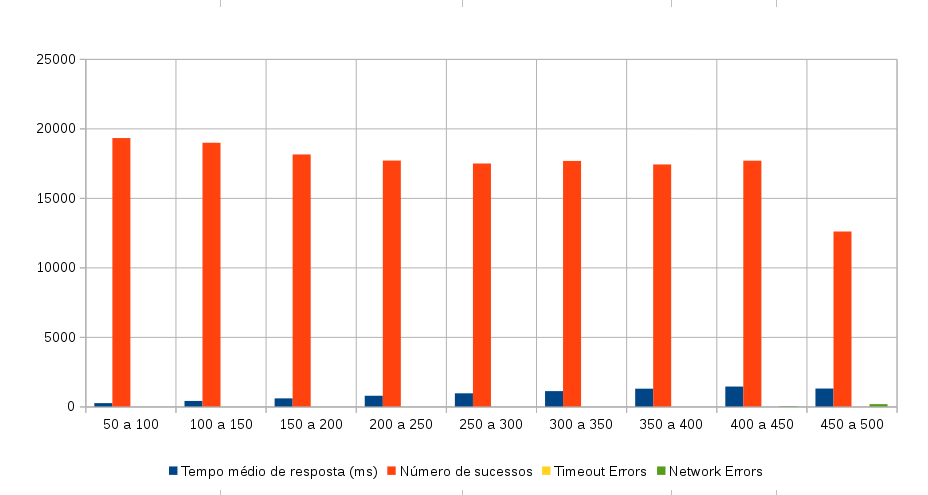
\includegraphics[width=.80\textwidth]{imagem/graficos/grafico_node_plano_de_teste_3.png}
    % Caption centralizada
    \captionsetup[grafico]{justification=centering}
    % Fonte
    \captionfont{\small{\textbf{\\Fonte: Autor}}}
  \end{grafico}

  No gráfico \ref{grafico:teste-mantendo-carga-usuario-node}  observa-se que o tempo de resposta da conexões 
  é muito baixo e o número de sucessos das conexões gira em torno de 17.429 sucessos. Os valores de tempo de resposta e
  número de sucessos somente decrecem quando executa o teste de 450 a 500 usuários. Neste teste houve um alto número de erros 
  de rede o qual influenciou diretamente no número de sucessos.
  
  Neste mesmo gráfico pode-se ver que o o número de erros de tempos de limite é sempre zero. Sendo assim podemos afirmar
  que não houve bloqueio nas operações de consulta a base de dados que poderiam impactar nos próximos testes.
  
  Comparando os dois gráficos \ref{grafico:teste-mantendo-carga-usuario-django} e \ref{grafico:teste-mantendo-carga-usuario-node} é
  visível a eficiência do protótipo em Node.Js pois em todos os campos o resultado obtido superou o primeiro protótipo.
  
  Pode-se concluir que o primeiro protótipo não tem condições de suportar grandes quantidades de usuários conectados ao
  sistema, visto o alto indíce de erros de limite de tempo excedido, baixo número de sucessos e tempo de resposta alto, 
  conforme exposto na tabela \ref{tab:sumario-resultado-plano-teste-a-3}. Para o protótipo Django o número ideal de usuarios
  conectados ao sistema fica em torno de 100 a 150 usuários enquanto em Node.Js tem-se 350 a 400 usuários conectados sem 
  erros.
  
  
% PÓS-TEXTUAIS %%
% Bibliografia no arquivo 'Dissertacao.bib'
% Alterar o título das referências para somente 'Referências'
\renewcommand{\bibname}{Referências}
\bibliographystyle{abnt-alf}
\bibliography{Dissertacao}

% Para forçar que os apêndices e anexos comecem no anverso
%\setboolean{@openright}{true}

\apendice
\begin{apendice}
%------------------------------------------------------------------------------------------------------------------------------------------------------
% Reiniciar numeração das figuras que aparecem no apêndice
\setcounter{figure}{0}

\chapter{Primeiro apêndice}
\label{apend:express-skel}

% Para diminuir espaçamento entre o título e o texto
\vspace{-1.9cm}

\lstinputlisting[
  language=c, 
  label=leitura-arquivos-diretorio-node, 
  caption={Fonte: \cite{pereira}. O inferno em chamadas de retorno}
]{pos-texto/leitura-arquivos-diretorio-node.js}

\lstinputlisting[
  language=c, 
  label=leitura-arquivos-diretorio-node-callback-heaven, 
  caption={Fonte: \cite{pereira}. Chamadas de retorno organizada}
]{pos-texto/leitura-arquivos-diretorio-node-callback-heaven.js}

\lstinputlisting[
  language=c, 
  label=leitura-arquivos-diretorio-node-strongloop, 
  caption={Fonte: \cite{strongloop}. Exemplo complexo de leitura de arquivos com callbacks hell}
]{pos-texto/leitura-arquivos-diretorio-node-strongloop.js}

\lstinputlisting[
  language=c, 
  label=leitura-arquivos-diretorio-node-strongloop-modular, 
  caption={Fonte: \cite{strongloop}. Exemplo complexo de leitura de arquivos modularizado}
]{pos-texto/leitura-arquivos-diretorio-node-strongloop-modular.js}

\lstinputlisting[
  language=c, 
  label=node-js-app, 
  caption={Fonte: Autor. Arquivo central para aplicação Node}
]{pos-texto/app.js}

\lstinputlisting[
  language=c,
  label=node-js-contact-route, 
  caption={Fonte: Autor. Módulo para a API de contato}
]{pos-texto/contacts.js}
\end{apendice}

\anexo
% Nome do Anexo
\chapter{Primeiro Anexo}
\label{primeiro-anexo}
% Para diminuir espa�amento entre o t�tulo e o texto
\vspace{-1.9cm}

% Texto
% Textos ou documentos não elaborados pelo autor.

\lstinputlisting[
  language=c, 
  label=leitura-arquivos-diretorio-node, 
  caption={Fonte: \cite{Pereira:2013}. O inferno em chamadas de retorno}
]{pos-texto/leitura-arquivos-diretorio-node.js}

\lstinputlisting[
  language=c, 
  label=leitura-arquivos-diretorio-node-callback-heaven, 
  caption={Fonte: \cite{Pereira:2013}. Chamadas de retorno organizada}
]{pos-texto/leitura-arquivos-diretorio-node-callback-heaven.js}

\lstinputlisting[
  language=c, 
  label=leitura-arquivos-diretorio-node-strongloop, 
  caption={Fonte: \cite{Strongloop:2013}. Exemplo complexo de leitura de arquivos com callbacks hell}
]{pos-texto/leitura-arquivos-diretorio-node-strongloop.js}

\lstinputlisting[
  language=c, 
  label=leitura-arquivos-diretorio-node-strongloop-modular, 
  caption={Fonte: \cite{Strongloop:2013}. Exemplo complexo de leitura de arquivos modularizado}
]{pos-texto/leitura-arquivos-diretorio-node-strongloop-modular.js}


\end{document}